\chapter{Problem Framework}

The problem of motion planning using an optimization-based approach is defined as follows:

The objective is to find a function
$\pi(t): [0,T] \to \mathcal{X}$, where $T$ represents the planning horizon and $\mathcal{X}$ is the configuration space, which defines the set of
feasible configurations for the vehicle.

The vehicle starts in an initial configuration $x_{\text{initial}} \in \mathcal{X}$, and the trajectory should end in a set of goal configurations
$X_{\text{goal}} \subset \mathcal{X}$.

Additionally, a constraint is defined over the derivatives of $\pi$ with respect to $t \in [0, T]$, denoted as $D(\pi(t), \pi'(t), \pi''(t), \dots)$.

To formulate an optimization problem, we define an objective function and a feasible set.

Let $\Pi[\mathcal{X}, T]$ represent the set of all possible functions mapping $[0, T]$ to $\mathcal{X}$.
Further, let $J(\pi): \Pi[\mathcal{X}, T] \to \mathbb{R}$ be the objective function.

\subsubsection{Problem Definition: Optimal Trajectory Planning}

Given a 6-tuple $(\mathcal{X}, x_{\text{initial}}, X_{\text{goal}}, D, J, T)$, the objective is to find:

\begin{align}
	x^* & = \underset{\pi \in \Pi(\mathcal{X},T)}{\operatorname{arg\,min}}
	J(\pi)                                                                                                                        \\ \text{s.t.
	}   & \quad \pi(0) = x_{\text{initial}}                                                                                       \\
	    & \quad \pi(T) \in X_{\text{goal}}                                                                                        \\
	    & \quad \pi(t) \in \mathcal{X},                                    & \text{for all} \quad t \in [0,T]                     \\
	    & \quad D(\pi(t), \pi'(t), \pi''(t), \dots),                       & \text{for all} \quad t \in [0,T] \label{eq:dynamics}
\end{align}

\section{Complexity}

Finding an exact solution in a dynamic environment is highly challenging.
The problem is inherently non-convex, and solvers cannot directly operate over a function space.

\section{Numerical Approach}

To address this problem numerically, we first define the constraints by modeling the vehicle and its environment.
We then reformulate the problem, discretize it, and approximate it.
Our goal is to obtain a solution that is both computationally efficient and reliable.

To achieve this, we employ a convex solver, necessitating adherence to disciplined convex programming (DCP) rules.

\section{Vehicle Models}

A vehicle model describes the position and orientation of the vehicle in the real world and predicts how these states change over time.
Different models vary in complexity and accuracy.
Generally, higher complexity results in increased accuracy.

Here, we introduce two fundamental models.

\subsection{State and Control Variables}

The state variables $x_i$ represent the current position and pose of the vehicle, potentially including velocity, steering angle, or other relevant
parameters.
We group these variables into a state vector $x$.

The control inputs $u_i$ are external influences that modify the state.
These are grouped into a control vector $u$.
Both $x$ and $u$ are time-dependent.

\subsection{Point Mass Model} \label{section:basic_pm}

The point mass model (PM) consists of four state variables:

\begin{equation}
	x = \begin{bmatrix} p_x \\ p_y \\ v_x \\ v_y \end{bmatrix}
	\label{eq:states_pm}
\end{equation}

Here, $p_x$ and $p_y$ represent the vehicle's position in a global fixed coordinate system.
Instead of an explicit orientation, velocity is divided into its components $v_x$ and $v_y$.

The model has two control inputs:

\begin{equation}
	u = \begin{bmatrix} a_x \\ a_y \end{bmatrix}
	\label{eq:controls_pm}
\end{equation}

These correspond to accelerations in the $x$ and $y$ directions.

The future position and velocity are determined by the following system of differential equations:

\begin{equation}
	\dot{x} = A x + B u
\end{equation}

where

\begin{equation}
	A = \begin{bmatrix} 0 & 0 & 1 & 0 \\ 0 & 0 & 0 & 1 \\ 0 & 0 & 0 & 0 \\ 0 & 0 & 0 & 0 \end{bmatrix}, \quad
	B = \begin{bmatrix} 0 & 0 \\ 0 & 0 \\ 1 & 0 \\ 0 & 1 \end{bmatrix}
\end{equation}

The control inputs are bounded by a circular constraint, where the radius $a_{\max}$ is a model parameter:

\begin{equation}
	\sqrt{u_1^2 + u_2^2} \leq a_{\max}
\end{equation}

This model is the simplest commonly used for motion planning.

\subsection{Kinematic Single Track Model}

The kinematic single track model (KST) consists of five state variables:

\begin{equation}
	x = \begin{bmatrix} p_x \\ p_y \\ \delta \\ v \\ \psi \end{bmatrix}
	\label{eq:states_kst}
\end{equation}

Similar to the point mass model, the first two state variables $p_x$ and $p_y$ define the vehicle's global position in a two-dimensional coordinate
system.
The vehicle is now modeled with an orientation $\psi$ relative to the global $x$-axis.
The velocity vector describes the velocity $v$ of the rear wheel, aligning with the orientation.
The front wheels can rotate around the yaw axis, and their angle relative to the orientation is represented by the steering angle $\delta$.

Two control inputs modify the velocity and steering, directly affecting the state variables:

\begin{equation}
	u = \begin{bmatrix} v_{\delta} \\ a_{\text{long}} \end{bmatrix}
	\label{eq:controls_kst}
\end{equation}
where $v_{\delta}$ is the steering velocity, and $a_{\text{long}}$ is the longitudinal acceleration.

The future state follows these differential equations:

\begin{align}
	 & \dot{p}_x = v\cos(\psi)                    \\
	 & \dot{p}_y = v\sin(\psi)                    \\
	 & \dot{\delta} = v_{\delta}                  \\
	 & \dot{v} = a_{\text{long}}                  \\
	 & \dot{\psi} = \frac{v}{l_{wb}} \tan(\delta) \\
\end{align}

The single-track name originates from simplifying front and rear wheels into single contact points, assuming no wheel slip, leading to a kinematic
model abstraction.
The following figure comprehends the whole model nicely.

\begin{figure}[h]
	\centering
	\begin{tikzpicture}
		% Axes
		\draw[->] (0,0) -- (2,0) node[right] {$x$};
		\draw[->] (0,0) -- (0,2) node[above] {$y$};

		% Rear Wheel
		\fill (2,2) circle (2pt); % Draws a small point at (2,2)

		% Vehicle body
		\draw[thick,rotate around={11.536959-90:(2,2)}] (1.8,1.3) rectangle (2.2,2.7);
		\draw[thick,rotate around={26.536959-90:(7,3)}] (6.8,2.3) rectangle (7.2,3.7);

		% Wheelbase
		\draw[-] (2,2) -- (7,3);
		\draw[dashed] (2,2) -- (1.7,3.5);
		\draw[dashed] (7,3) -- (6.7,4.5);
		\draw[dashed, <->] (1.8,3) -- (6.8,4) node[midway,above] {$l_{wb}$};

		% Velocity vector
		\draw[->] (2,2.1) -- (4,2.5) node[midway,above] {$v$};

		% Heading angle
		\draw[dashed] (3.25,2.25) -- (6,2.25);
		\draw[->] (6,2.25) arc (0:11.536959:2.75);
		\node at (5.7,2.5) {$\psi$};

		% Steering angle
		\draw[dashed] (7,3) -- (8.5,3.3);
		\draw[dashed] (7,3) -- ++(26.536959:1.5);
		\draw[->] (8.5,3.3) arc (11.536959:26.536959:1.5);
		\node at (8.2,3.43) {$\delta$};

		% Displacement vector
		\draw[dashed,thick,->] (0,0) -- (1.95,1.95)
		node[midway, left, shift={(-0,+0.4)}] {$\begin{bmatrix}s_x \\ s_y \end{bmatrix}$};
	\end{tikzpicture}
	\caption{Bicycle model representation of a vehicle.}
	\label{fig:bicycle_model}
\end{figure}

The following additional constraints are part of the model, a parameter $a_{max}$ is introduced:

\begin{equation}
	\sqrt{u_2^2 + (x_4\dot{x}_5)^2} \leq a_{\max}
\end{equation}

For both models, the vehicle is additionally constrained by its velocity range, steering angle range, and the rate of change of the steering angle.
These constraints are natural and should not be overlooked.

\section{Constraints}

The constraints on the derivatives defined in \eqref{eq:dynamics}, using one of the models, can be expressed as:

\begin{equation}
	\pi'(t) = f(\pi(t), u(t))
\end{equation}

\section{Problem Reformulation}

Since solvers cannot operate directly on function spaces, the first step is to approximate the infinite-dimensional space of trajectories using a
finite-dimensional vector space.
Additionally, we transform the constraints, originally defined by set membership and predicates, into a system of equalities and inequalities, which
are compatible with standard solver inputs.

An alternative approach involves using penalty or barrier functions to incorporate constraints into the objective function.

\subsection{Direct vs.
	Indirect Methods}

\subsubsection{Direct Methods}

To project the function space into a finite-dimensional
vector space, we define a set of basis functions that span a subspace of the original space.
A function in this subspace is then represented as a linear combination of the basis functions:

\begin{equation}
	\tilde{\pi}(t) = \sum_{i=1}^{N} \pi_i \phi_i(t)
\end{equation}

While this approach restricts the search space, potentially deviating from the true optimal solution, it allows for numerical tractability.
One of the most widely used techniques for trajectory approximation is numerical integration with collocation.
In this approach, the trajectory is required to satisfy the constraints at a discrete set of time points $\{t_i\}_{i=1}^{m}$.
Numerical integration techniques are then employed to approximate the trajectory between these points.

\subsection{Discrete-Time Problem Formulation}

Using direct methods, we now reformulate the optimization problem over a finite-dimensional vector space.

Let $\mathcal{X}$ be the set of valid vehicle states and $\mathcal{U}$ the set of all feasible control inputs.

The trajectory is defined at discrete time points $\{t_i\}_{i=1}^{m}$, where $\pi(t_i) = x_i$.
The objective function is then defined over $\mathcal{X} \times \mathcal{U}$ as $J: \mathcal{X} \times \mathcal{U} \to \mathbb{R}$.

\subsubsection{Problem Definition: Discrete-Time Optimal Trajectory Planning}

Given a 7-tuple $(\mathcal{X}, \mathcal{U}, x_{\text{initial}}, X_{\text{goal}}, f, J, \{t_i\}_{i=1}^{m})$, the objective is to find:

\begin{align}
	u^* & = \underset{u \in \mathcal{U}^{T-1}}{\operatorname{arg\,min}} \sum_{i=1}^{T-1}
	J(x_{i+1}, u_{i})                                                                                                                                      \\ \text{s.t.
	}   & \quad x_1 = x_{\text{initial}}                                                                                                                   \\
	    & \quad x_T \in X_{\text{goal}} \subseteq \mathcal{X}                                                                                              \\
	    & \quad (x_i, u_i) \in \mathcal{C} \subseteq \mathcal{X} \times \mathcal{U}      & \forall i \in \{1, \dots, m-1\} \label{eq:coupling_constraints} \\
	    & \quad x_{i+1} = x_i + (t_{i+1} - t_i) f(x_i, u_i)                              & \forall i \in \{1, \dots, m-1\} \label{eq:discrete_dynamics}
\end{align}

Given an initial state $x_{\text{initial}}$ and a control sequence over the time horizon, we use the vehicle model dynamics $f$ and numerical
integration to compute the state at each time step.
This formulation introduces a coupling constraint $\mathcal{C}$ that governs the relationship between state and control inputs.

One challenge is that this formulation does not yet conform to disciplined convex programming (DCP) principles.
We will address this issue by discussing applicable modeling techniques, including approximations and their implications, focusing first on the point
mass model.

\section{Frenet Frame Representation}

In our previous models, vehicle positions and orientations were represented using a global Cartesian coordinate system.
While this approach is effective for modeling vehicle dynamics, it becomes cumbersome when incorporating road topology constraints.

Since road topology is typically known in advance, we can leverage this knowledge to define a coordinate system that simplifies constraint modeling.
The Frenet frame provides a more intuitive way to describe vehicle motion relative to a reference path, resulting in a more structured and often
convex constraint representation.

The Frenet frame consists of two coordinates, $(s, n)$, where $s$ represents the arc-length position along the reference curve, and $n$ denotes the
orthogonal deviation from it.
This transformation allows constraints to be naturally aligned with the road structure, simplifying feasibility checks and trajectory optimization.

\begin{figure}[h]
	\centering
	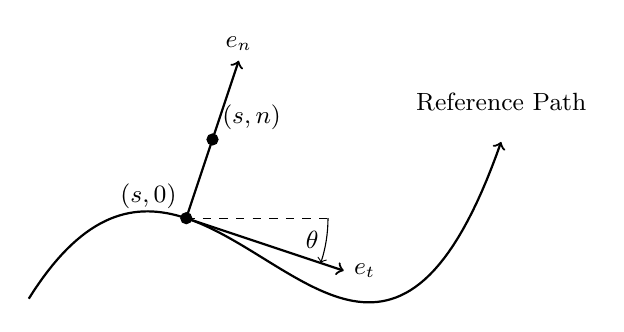
\begin{tikzpicture}
		% Draw the reference path (a smooth curve)
		\draw[->, thick, domain=2:8, samples=100] plot (\x, {-5 + 4.466667*(\x) - 0.7444444*(\x)^2 - 0.005555556*(\x)^3 + 0.005555556*(\x)^4});

		% Label the reference path
		\node[black] at (8,3.5) {\small Reference Path};

		% Point on the reference path
		\filldraw[black] (4,2.022224352) circle (2pt);
		\node[above left] at (4,2.022224352) {\small $(s, 0)$};

		% Draw tangent and normal vectors
		\draw[->, thick] (4,2.022224352) -- (6,1.3555515519999999) node[right] {\small $e_t$};
		\draw[->, thick] (4,2.022224352) -- (4.6666728,4.022224352) node[above] {\small $e_n$};

		% Theta angle
		\draw[dashed] (4,2.022224352) -- (5.8,2.022224352);
		\draw[->] (5.8,2.022224352) arc (0:-18.43510695912798:1.8);
		\node at (5.6,1.75) {\small $\theta$};

		% Off-path point (s, n)
		\filldraw[black] (4.333336399999999,3.022224352) circle (2pt);
		\node[above right] at (4.333336399999999,3.022224352) {\small $(s, n)$};
	\end{tikzpicture}
	\caption{Frenet Frame Representation}
	\label{fig:frenet_frame}
\end{figure}

Let $\theta(s)$ denote the angle between the tangent vector at position $s$ along the reference path and the $x$-axis of a global fixed coordinate
system.
If the global position of the reference path at the starting point $s_{\min}$ is known, the global coordinates of any point along the reference path can be determined using:

\begin{align}
	p_x(s) & = \int_{s_{\min}}^{s} \cos(\theta(\sigma)) d\sigma + p_x(s_{\min}), \\
	p_y(s) & = \int_{s_{\min}}^{s} \sin(\theta(\sigma)) d\sigma + p_y(s_{\min}).
\end{align}

The reference path is aligned with the road, allowing the vehicle's position to be described within this Frenet frame.
In the following section, we will transition the point mass model's dynamics into this coordinate system.

\subsection{Body-Fixed Coordinate System}

To further refine the vehicle's representation, we introduce the body-fixed coordinate system, which is attached to the moving reference position of
the vehicle within the global coordinate system.
The first axis of the body-fixed coordinate system aligns with the vehicle's longitudinal orientation and is denoted by the unit vector $e_{b,x}$.
The second axis is orthogonal to the first and is denoted by $e_{b,y}$.
This coordinate system simplifies modeling control inputs and forces acting on the vehicle.

